\chapter{Abbildungen, Tabellen, Quellkode}
\label{chap:Abbildungen}

\section{Allgemeines}

Abbildungen (\emph{figures}) und Tabellen (\emph{tables}) werden üblicherweise
zusammen mit einem nummerierten Titel (\emph{caption}) zentriert
angeordnet (siehe Abb.~\ref{fig:urlaub}).
Im Text \emph{muss} es zu jeder Abbildung einen Verweis geben und die eigentliche Abbildung
sollte erst \emph{nach} dem ersten Verweis platziert werden.

\begin{figure}
\centering
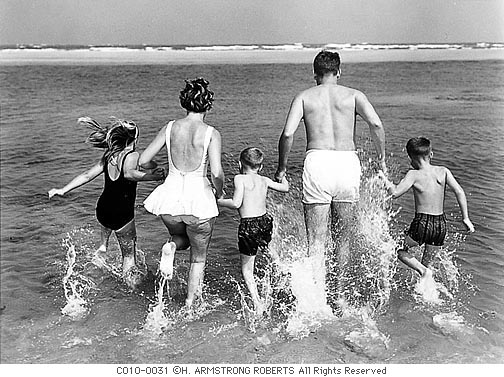
\includegraphics[width=.85\textwidth]{CS0031}
\caption{Newport Beach 1957.}
\label{fig:urlaub}
\end{figure}



\section{\emph{Let Them Float!}}

Das Platzieren von Abbildungen und Tabellen gehört zu den
schwierigsten Aufgaben im Schriftsatz, weil diese meist viel Platz
benötigen und häufig nicht auf der aktuellen Seite im laufenden
Text untergebracht werden können. Diese Elemente müssen daher an
eine geeignete Stelle auf nachfolgenden Seiten verschoben werden,
was manuell sehr mühsam (jedoch in \emph{Word} beispielsweise unerlässlich) ist.

In \latex funktioniert das weitgehend automatisch, indem
Abbildungen, Tabellen und ähnliche als "`Floating Bodies"'
behandelt werden. Bei der Positionierung dieser Elemente wird
versucht, einerseits im Textfluss möglichst wenig Leer\-raum
entstehen zu lassen und andererseits die Abbildungen und Tabellen
nicht zu weit von der ursprünglichen Textstelle zu entfernen.

Der Gedanke, dass etwa Abbildungen kaum jemals genau an der
ge\-wünsch\-ten Stelle und möglicherweise nicht einmal auf
derselben Seite Platz finden, ist für viele Anfänger aber offenbar sehr
ungewohnt oder sogar beängstigend. Dennoch sollte man zunächst einmal
getrost \latex\ diese Arbeit überlassen und \emph{nicht} manuell
eingreifen. Erst am Ende, wenn das gesamte Dokument "`steht"' und
man mit der automatischen Platzierung wirklich nicht zurande
kommt, sollte man (durch gezielte Platzierungsanweisungen
\cite[S.~33]{Oetiker01}) \textbf{in Einzelfällen} eingreifen.



\section{Captions}

Bei Abbildungen steht der Titel üblicherweise \emph{unten}, bei
Tabellen hingegen -- je nach Konvention -- \emph{oben} (wie in diesem Dokument) 
oder ebenfalls \emph{unten}. In \latex\ erfolgt
auch die Nummerierung der Abbildungen automatisch, ebenso der
Eintrag in das (optionale)
Abbildungsverzeichnis%
\footnote{Ein eigenes Verzeichnis der Abbildungen am Anfang des Dokuments
ist zwar leicht erstellt, in einer Diplomarbeit aber (und eigentlich
überall sonst auch) überflüssig. Man sollte es daher weglassen.}
am Beginn des Dokuments.

Die Markierung der Captions%
\footnote{Ausnahmsweise wird das Wort "`Caption"' im Folgenden
ohne deutsche Übersetzung verwendet.} erfolgt in \latex mithilfe
der \verb!\label{}! Anweisung, die unmittelbar auf die
\verb!\caption{}! Anweisung folgen muss:
%
\begin{LaTeXCode}
\begin{figure}
\centering
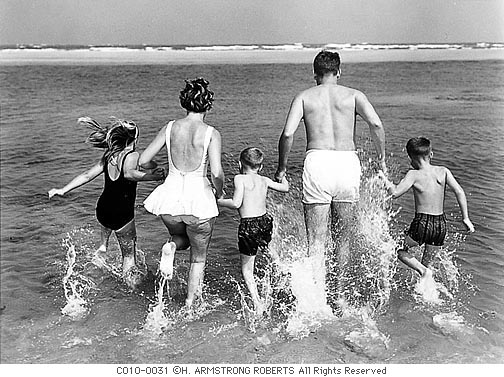
\includegraphics[width=.85\textwidth]{CS0031}
\caption{Newport Beach 1957.}
\label{fig:urlaub}
\end{figure}
\end{LaTeXCode}
%
Der Name des Labels (\texttt{fig:urlaub}) kann beliebig gewählt werden. 
Die Kennzeichnung \texttt{fig:} ist (wie in Abschn.\ \ref{sec:querverweise} 
erwähnt) nur eine nützliche Hilfe, um beim Schreiben verschiedene Arten 
von Labels besser unterscheiden zu können.

Die Länge der Captions kann dabei sehr unterschiedlich sein. Je
nach Anwendung und Stil ergibt sich manchmal eine sehr kurze
Caption (Abb.~\ref{fig:urlaub}) oder eine längere
(Abb.~\ref{fig:univac}).
Man beachte, wie bei kurzen Captions ein
zentrierter Satz und bei langen Captions ein Blocksatz verwendet
wird (\latex macht das automatisch).
Captions sollten \emph{immer} mit einem Punkt abgeschlossen sein.%
\footnote{Kurioserweise verlangen manche Anleitungen
genau das Gegegenteil, angeblich, weil beim klassischen Bleisatz 
die abschließenden Punkte im Druck häufig "`weggebrochen"' sind. 
Das kann man glauben oder nicht, im Digitaldruck 
spielt es jedenfalls keine Rolle.}

\begin{figure}
\centering
\FramePic{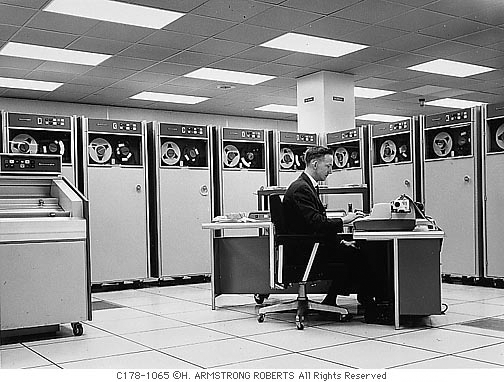
\includegraphics[width=.85\textwidth]{CS1065}}
\caption{Beispiel für einen langen Caption-Text. \textsc{Univac}
brachte 1961 mit dem Modell 751 den ersten Hochleistungsrechner
mit Halbleiterspeicher auf den Markt. Von diesem Computer wurden
in den U.S.A.\ bereits im ersten Produktionsjahr über fünfzig
Exemplare verkauft, vorwiegend an militärische Dienststellen,
Versicherungen und Großbanken. Die Ablöse erfolgte zwei Jahre
später durch das zusammen mit \textsc{Sperry} entwickelte Modell 820.
Das klingt vielleicht plausibel, ist aber frei erfunden und
vermutlich völliger Unsinn.} 
\label{fig:univac}
\end{figure}





\section{Abbildungen}

Für die Einbindung von Grafiken in \latex wird die Verwendung des Stan\-dard-Pakets
\texttt{graphicx}\footcite{Carlisle99} empfohlen 
(wird durch das \texttt{htl}-Paket bereits eingebunden). 
Folgende Bildformate können verwendet werden:
%
\begin{center}
\begin{tabular}{|l|l|l|}
\hline
Rasterbilder:    & PNG, JPEG, PDF \\
\hline
Vektorgraphiken: & PDF \\
\hline
\end{tabular}
\end{center}
%

\subsection{Wo liegen die Grafikdateien?} 

Die Bilder werden üblicherweise in einem Unterverzeichnis (oder in mehreren Unterverzeichnissen) abgelegt,
im Fall dieses Dokuments in \url{images/}.
Dazu dient die folgende Anweisung
am Beginn des Hauptdokuments \url{Diplomarbeit.tex} (\sa\ Anhang
\ref{app:latex}):
%
\begin{quote}\small
\verb!\graphicspath{{images/}}!
\end{quote}
%
Der (zum Hauptdokument relative) Pfad \texttt{graphicspath} kann innerhalb des
Dokuments jederzeit geändert werden, was durchaus nützlich ist, wenn man
\zB\ die Grafiken einzelner Kapitel getrennt in entsprechenden Verzeichnissen
ablegen möchte.
Die Größe der Abbildung im Druck kann durch Vorgabe einer bestimmten
Breite oder Höhe oder eines Skalierungsfaktors gesteuert werden, {\zB}:
%
\begin{quote}\small
\verb!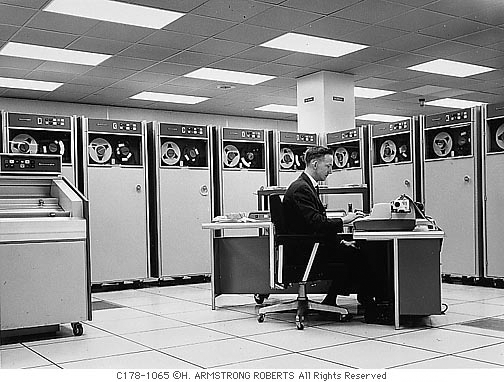
\includegraphics[width=.85\textwidth]{CS1065}! \\
\verb!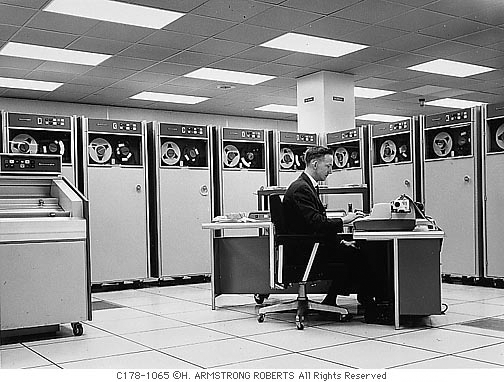
\includegraphics[scale=1.5]{CS1065}!
\end{quote}
%
Man beachte, dass dabei die Datei-Extension nicht explizit angegeben werden muss. 
Das ist \va\ dann praktisch, wenn man verschiedene Workflows mit jeweils
unterschiedlichen Dateitypen verwendet.


\subsection{Grafiken einrahmen} 

Mit dem Makro \verb!\FramePic{}! (definiert in \texttt{htl.sty}) kann man
optional einen dünnen Rahmen rund um die Grafik erzeugen, \zB:
%
\begin{quote}\small
\verb!\FramePic{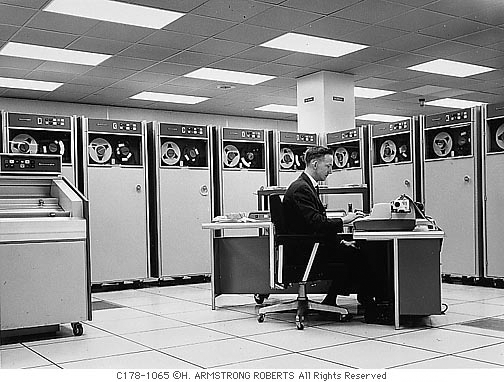
\includegraphics[height=50mm]{CS1065}}!
\end{quote}
%
Das wird man üblicherweise nur bei Rasterbildern tun, insbesondere wenn sie zum Rand hin sehr hell sind
und ohne Rahmen nicht vom Hintergrund abgrenzbar wären.

\subsection{Rasterbilder (Pixelgrafiken)}

Generell sollte man Bilder bereits vorher so aufbereiten,
dass sie später beim Druck möglichst wenig an Qualität verlieren.
Es empfiehlt sich daher, die Bildgröße (Auflösung) bereits im Vorhinein
(\zB mit \emph{Photoshop})
richtig einzustellen.
Brauchbare Auflösungen bezogen auf die endgültige Bildgröße sind:
%
\begin{itemize}
  \item \textbf{Farb- und Grauwertbilder:} 150--300 dpi
  \item \textbf{Binärbilder (Schwarz/Weiß):} 300--600 dpi
\end{itemize}
%
Eine wesentlich höhere Auflösung macht aufgrund der beim Laserdruck notwendigen
Rasterung keinen Sinn, auch bei 1200 dpi-Druckern.
Speziell \emph{Screen\-shots} sollte man nicht zu klein darstellen,
da sie sonst schlecht lesbar sind (max.\ 200 dpi, besser 150 dpi).
Dabei ist zu bedenken, dass die Arbeit auch als Kopie in allen
Details noch gut lesbar sein sollte.

\subsubsection{JPEG-Problematik}

Keinesfalls sollte man Bilder, die für den Einsatz in
Druckdokumenten gedacht sind, mit verlustbehafteten
Kompressionsverfahren abspeichern. Insbesondere sollte man die Verwendung
von JPEG möglichst vermeiden, auch wenn viele Dateien dadurch
wesentlich kleiner würden. 
Eine Ausnahme ist, wenn die Originaldaten nur in JPEG vorliegen und für die 
Einbindung nicht bearbeitet oder verkleinert wurden. Ansonsten sollte man immer
PNG verwenden.

Besonders gerne werden farbige \textbf{Screenshots} einer JPEG-Kompression%
\footnote{Das JPEG-Verfahren ist für natürliche Fotos konzipiert und dafür auch gut geeignet,
seine undifferenzierte Verwendung ist aber zu einer globalen Plage geworden.}
unterzogen, obwohl deren verheerende Folgen auch für jeden Laien sichtbar sein sollten
(Abb.~\ref{fig:jpeg-pfusch}).

\begin{figure}
\centering\small
\begin{tabular}{cc}
\FramePic{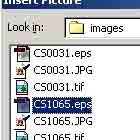
\includegraphics[width=0.45\textwidth]{screenshot-dirty}} &		% JPEG file
\FramePic{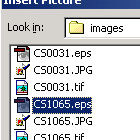
\includegraphics[width=0.45\textwidth]{screenshot-clean}} \\	% PNG file
(a) & (b) 
\end{tabular}
\caption{Typischer JPEG-Pfusch. Screenshots und ähnliche im Original
verfügbare Rasterbilder sollten für Druckdokumente \emph{keinesfalls} mit
JPEG komprimiert werden. Das Ergebnis (a) sieht gegenüber dem
unkomprimierten Original (b) nicht nur schmutzig aus, sondern wird
auch schnell unleserlich.} 
\label{fig:jpeg-pfusch}
\end{figure}






\subsection{Vektorgrafiken}

Für schematische Abbildungen (\zB Flussdiagramme, Entity-Relationship-Diagramme
oder sonstige strukturelle Darstellungen) sollte man unbedingt
Vektorgrafiken verwenden.
Gerasterte Grafiken, wie man sie üblicherweise als GIF- oder PNG-Dateien
auf Webseiten findet, haben in einem Druckdokument nichts zu suchen, notfalls
muss man sie mit einem entsprechenden Werkzeug \emph{neu} zeichnen (natürlich
unter Angabe der ursprünglichen Quelle).

In diesem Fall kommt als Datenformat nur PDF in Frage,
dieses bietet sich aber auch in anderen Umgebungen als universelles
Vektor-Format an.
Zur Erstellung von PDF-Vektorgrafiken benötigt man ein geeignetes
Grafikprogramm, \zB\ \emph{Freehand} von \emph{Macromedia}
oder \emph{Illustrator} von \emph{Adobe}.
Manche gängige Grafikprogramme 
unterstützen allerdings keinen direkten Export von PDF-Dateien
oder erzeugen unbrauchbare Dateien. Vor der Entscheidung
für eine bestimmte Zeichensoftware sollte man das im Zweifelsfall
ausprobieren.
PDF kann im Notfall über einen entsprechenden Druckertreiber erzeugt werden.




\subsubsection{Einbettung von Schriften}

Die Wiedergabe von Textelementen ist abhängig von der auf dem
Computer (oder Drucker) installierten Schriften und der Form der
Schrifteinbettung im Quelldokument. Die korrekte Darstellung am
Bildschirm eines Computers bedeutet nicht, dass dasselbe Dokument
auf einem anderen Computer oder Drucker genau so dargestellt wird.
Dieser Umstand ist besonders wichtig, wenn Druckdokumente online
zur Verfügung gestellt werden. Kontrollieren Sie daher genau, ob
die innerhalb Ihrer Grafiken verwendeten Schriften auch exakt wie
beabsichtigt im Ausdruck aufscheinen.


\subsubsection{Strichstärken -- \emph{Hairlines} vermeiden!}

In Grafik-Programmen wie \emph{Freehand} und \emph{Illustrator},
die sich im Wesentlichen an der \emph{PostScript}-Funktionalität
orientieren, ist es möglich, Linien bzgl.\ ihrer Stärke als
"`Hairline"' zu definieren. Im zugehörigen \emph{PostScript}-Kode
wird dies als \texttt{linewidth} mit dem Wert \texttt{0} ausgedrückt und
sollte am Ausgabegerät "`möglichst dünne"' Linien ergeben. Das
Ergebnis ist ausschließlich vom jeweiligen Drucker
abhängig und somit kaum verhersagbar. 
\textbf{Fazit:} Hairlines vermeiden und stattdessen immer konkrete
Strichstärken ($\geq 0.25 \mathrm{pt}$) einstellen!


\subsection{\tex-Schriften auch in Grafiken?}
\label{sec:tex-schriften-in-grafiken}

Während man sich bei Abbildungen, die mit externen
Grafik-Programmen erzeugt werden, meist mit ähnlich aussehenden
Schriften (wie \emph{Times-Roman} oder \emph{Garamond}) abhilft,
besteht bei Puristen oft der verständliche Wunsch, die 
\emph{Computer-Modern} (CM) Schriftfamilie von {\tex}/{\latex} auch
innerhalb von eingebetteten Grafiken einzusetzen.

\subsubsection{\emph{BaKoMa}-Schriften}

Glücklicherweise stehen einige Portierungen von CM als {\em
TrueType}-Schriften zur Verfügung, die man auch in herkömmlichen
DTP-Anwendungen unter \emph{Windows} und \emph{Mac~OS} verwenden
kann. Empfehlenswert ist \va\ die \emph{BaKoMa Fonts
Collection}\footnote{Von Basil K.\ Malyshev -- die BaKoMa-Fonts
liegen dieser Vorlage bei, ansonsten findet man sie \zB\ unter
\url{www.ctan.org/tex-archive/fonts/cm/ps-type1/bakoma/}.}, die
neben den CM-Standardschriften auch die mathematischen Schriften
der AMS-Familie ent\-hält und zudem kostenfrei ist. Natürlich
müssen die TrueType Schriften vor der Verwendung zunächst auf dem
eigenen PC installiert werden.


\subsection{Abbildungen mit mehreren Elementen}

Werden mehrere Bilder oder Grafiken zu einer Abbildung zusammengefasst, 
verwendet man üblicherweise eine gemeinsame Caption, wie in Abb.~\ref{fig:Bearings}
dargestellt. Im Text könnte ein Verweis auf einen einzelnen Teil der Abbildung, etwa das 
einreihige Rollenlager in Abb.~\ref{fig:Bearings}\thinspace(c), so aussehen:
%
\begin{itemize}
\item[] \verb!Abb.~\ref{fig:Bearings}\thinspace(c)! 
\end{itemize}
%
Für kompliziertere Abbildungen sollte man die Verwendung des 
\texttt{subcaption}-Pakets \footcite{Cochran95} in Betracht ziehen. Ein Beispiel ist in der Vorlage in Abbildung \ref{fig:Settings} zu finden.


\subsection{Quellenangaben in Captions}
\label{sec:QuellenangabenInCaptions}

Wenn Bilder, Grafiken oder Tabellen aus anderen Quellen verwendet werden, dann muss ihre Herkunft in jedem Fall klar ersichtlich gemacht werden, und zwar am besten direkt in der Caption.
Verwendet man beispielsweise eine Grafik aus einem Buch oder einer sonstigen zitierfähigen Publikation, dann sollte man diese in das Literaturverzeichnis aufnehmen und wie üblich zitieren, wie in Abb.\ \ref{fig:Bearings} demonstriert. Da Grafiken floating-Elemente sind, muss statt mit
\verb!\footcite{..}! die Kombination \verb!\footnotemark! und \verb!\footcitetext! verwendet werden. Weitere Details zu dieser Art von Quellenangaben finden sich in Kap.\ \ref{cha:Literatur}.

Bei Bildern aus dem Internet ist es hingegen ratsam, die zugehörige Website \emph{nicht} in das Literaturverzeichnis aufnehmen, sondern (mit \verb!\url{..}!) direkt in der Caption oder in einer Fußnote anzugeben (siehe Abschn.\ \ref{sec:OnlineQuellen} und Abbildung \ref{fig:latexinternet}). 

Sollte die Kombination von Caption, Fußnote und Url verwendet werden, muss die Fußnote in ein \verb!\footnotemark! und ein \verb!\footnotetext! aufgeteilt werden. Abbildung \ref{fig:latexinternet} zeigt ein Beispiel davon und das Programm \ref{prog:footnotemark} zeigt den \latex\ Quelltext. Die Fußnote wird in diesem Fall nicht immer auf der selben Seite wie die Abbildung sein, was durch die Durchnumerierung der Fußnoten jedoch kein Problem darstellen sollte. Vor allem, da die Fußnote sich dann auf der Seite befindet wo die Abbildung im Text erwähnt werden sollte. 

\begin{program}
% place caption consistently either at the top or bottom:
\caption{\latex\ Quelltext zu Abbildung \ref{fig:latexinternet}.}
\label{prog:footnotemark}
%
\begin{LaTeXCode}
\begin{figure}
\centering

\includegraphics[width=.85\textwidth]{LatexInternet}
\caption[]{Witze über Latex im Internet.\footnotemark }
\label{fig:latexinternet}
\end{figure}
\footnotetext{Quelle: \url{https://pr0gramm.com/static/1454890}}
\end{LaTeXCode}
%
\end{program}

% Beispiel für die Verwendung von "subfigure"

\begin{figure}
\centering\small
\begin{tabular}{cc}
  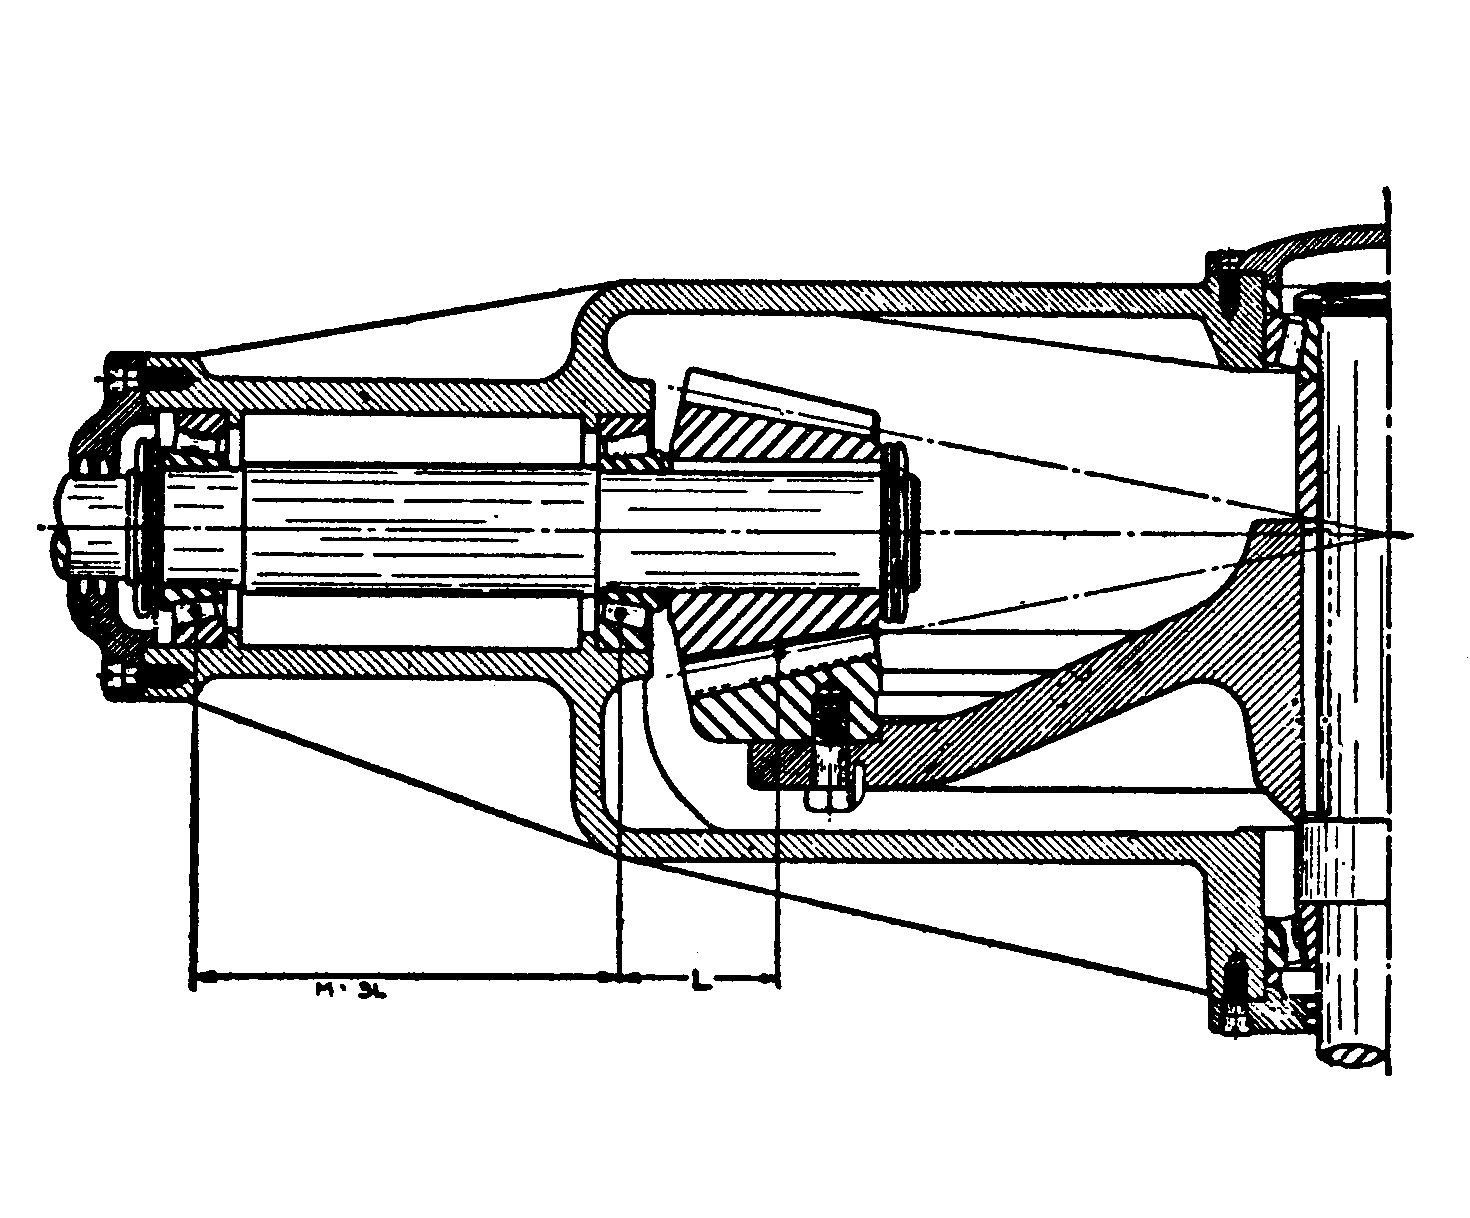
\includegraphics[width=.45\textwidth]{overhang-mounting} &
  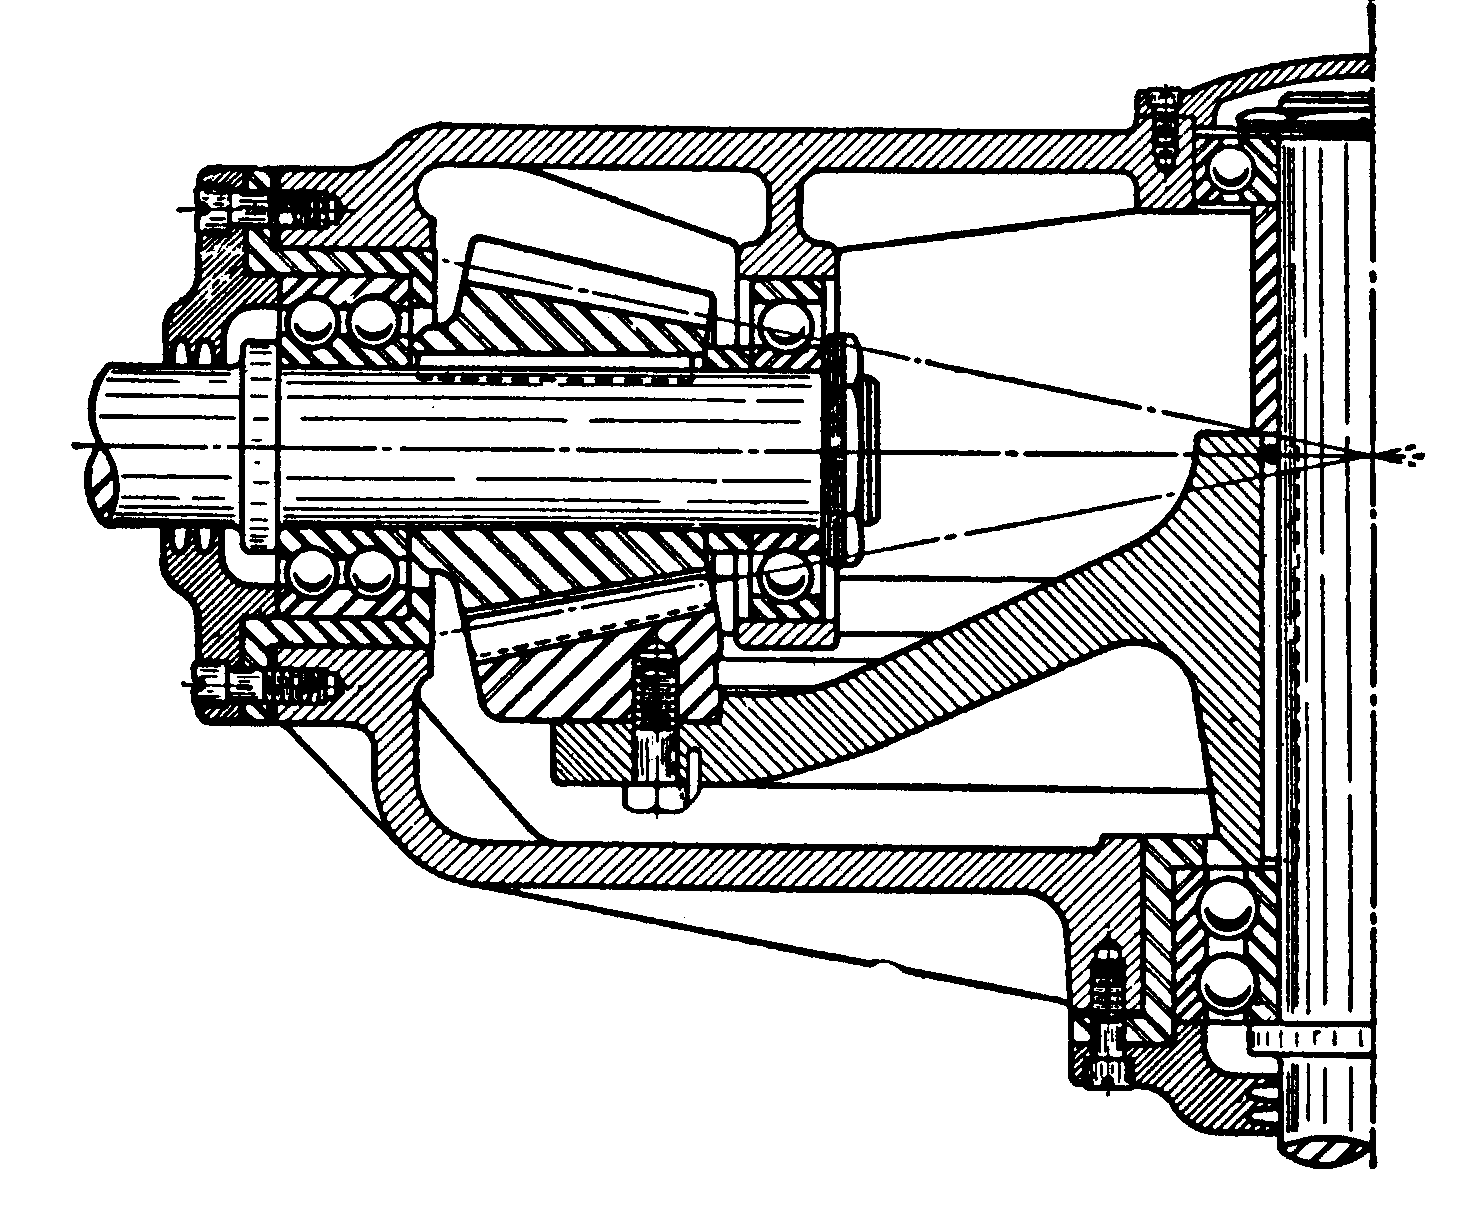
\includegraphics[width=.45\textwidth]{straddle-mounting} \\
  (a) & (b)
\\[4pt]	%vertical extra spacing (4 points)
  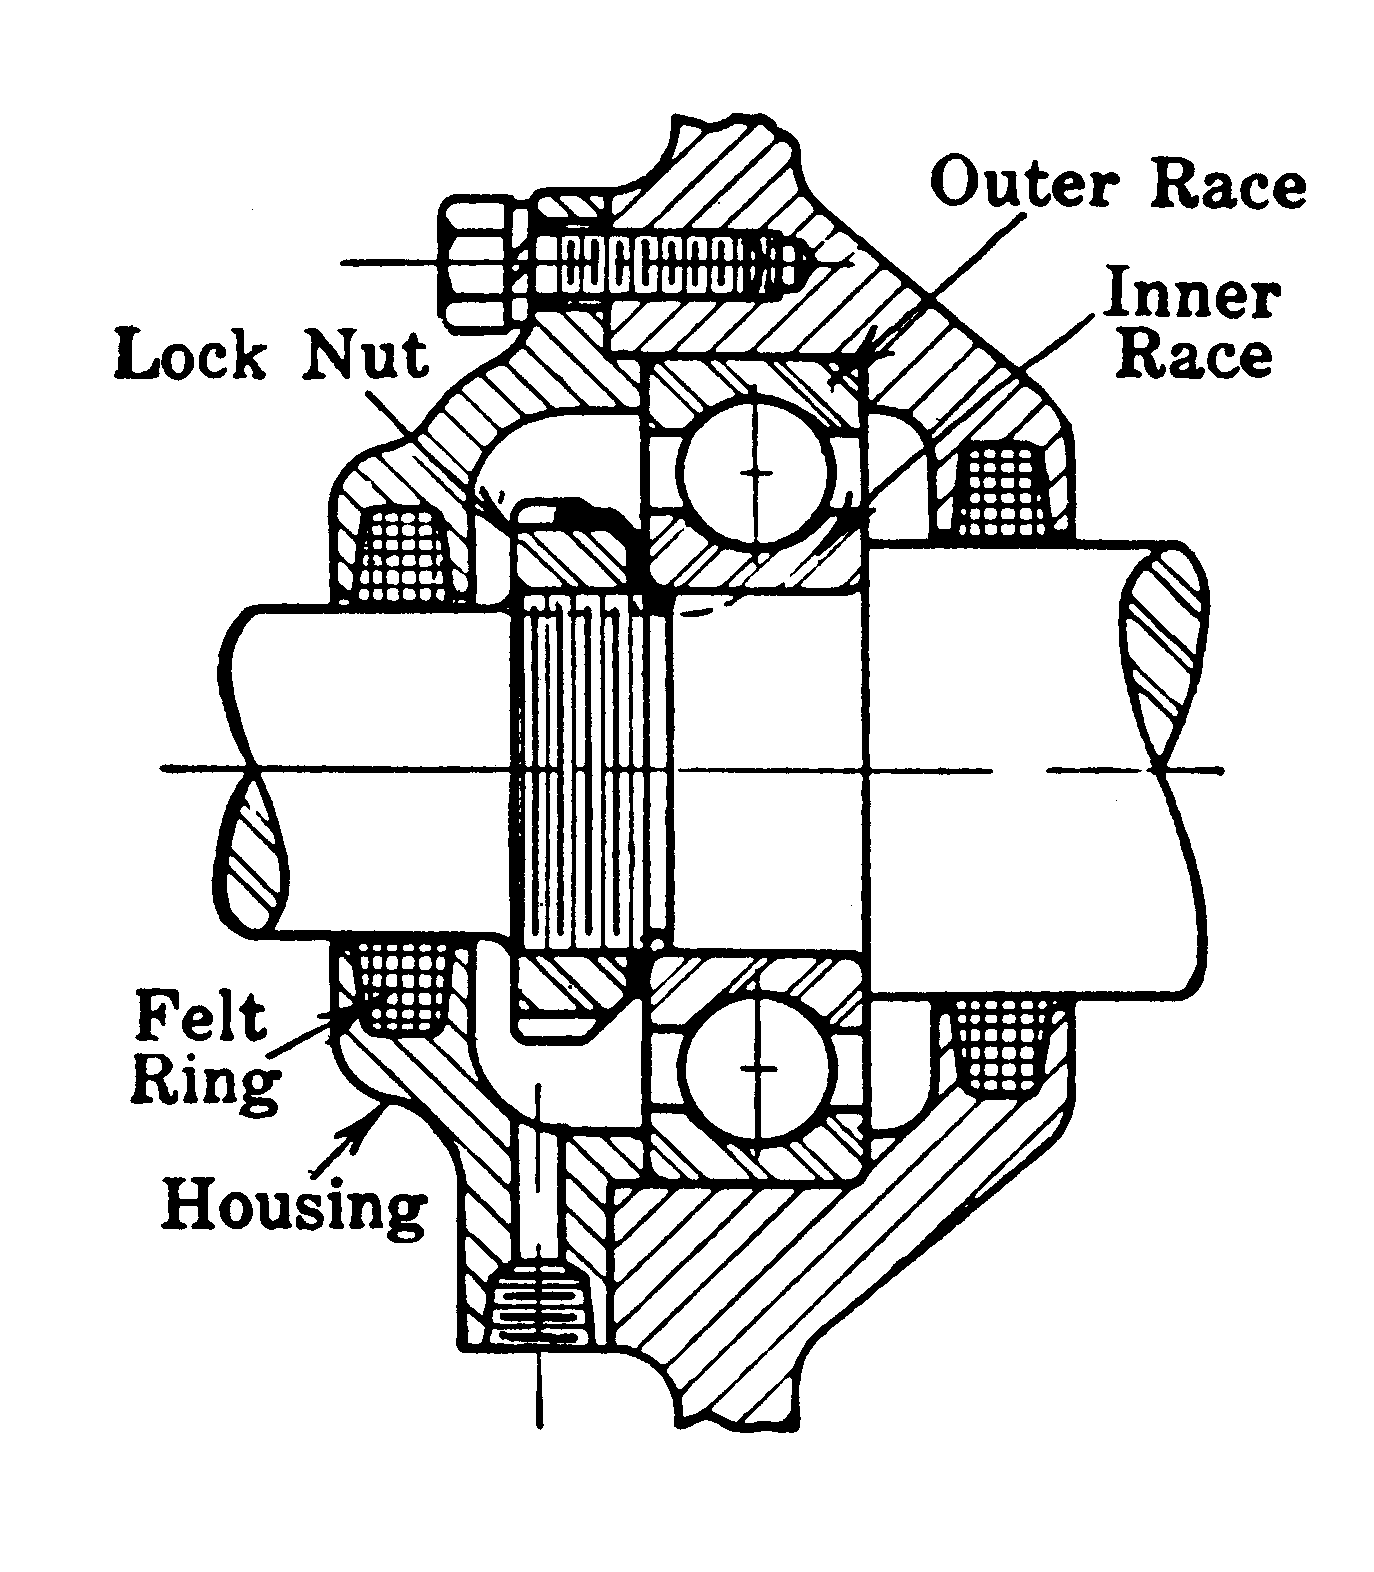
\includegraphics[width=.45\textwidth]{ball-bearing-1} &
  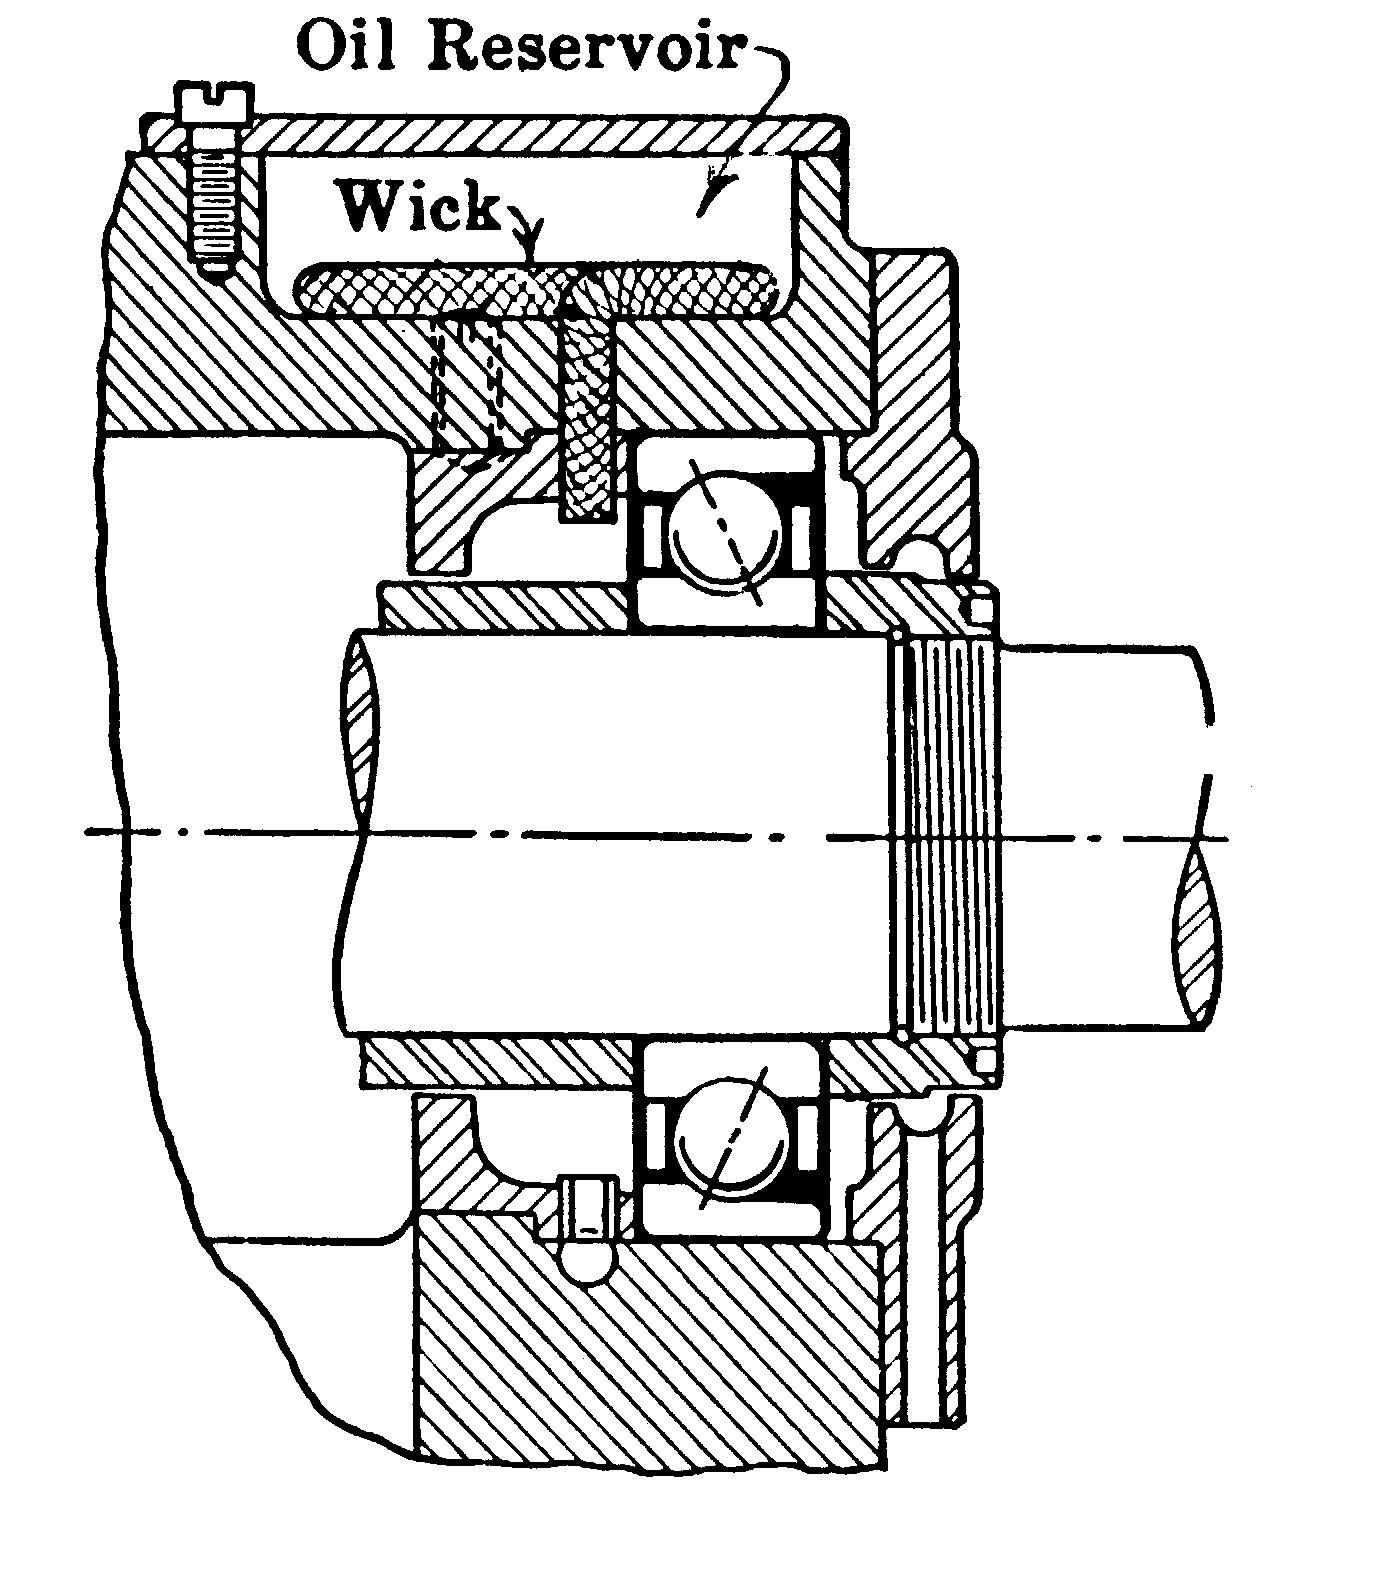
\includegraphics[width=.45\textwidth]{ball-bearing-2} \\
  (c) & (d)
\end{tabular}
%
\caption[]{Diverse Maschinenelemente.
Overhang Mounting (a), Straddle Mounting (b),
einreihiges Rollenlager (c), Schmierung von Rollenlagern (d).
Aus \citetitle{Faires34}.\footnotemark }
\label{fig:Bearings}
\end{figure}
\footcitetext{Faires34}

\begin{figure}
\centering

\includegraphics[width=.85\textwidth]{LatexInternet}
\caption[]{Witze über Latex im Internet.\footnotemark }
\label{fig:latexinternet}
\end{figure}
\footnotetext{Quelle: \url{https://pr0gramm.com/static/1454890}}

\section{Tabellen}

Tabellen werden häufig eingesetzt um numerische Zusammenhänge, Testergebnisse
etc.\ in übersichtlicher Form darzustellen.
Ein einfaches Beispiel ist Tab.~\ref{tab:processors}, der \latex-Quelltext dazu
findet sich in Prog.~\ref{prog:processors-source}.


\begin{table}
\caption{Prozessor-Familien im Überblick.}
\label{tab:processors}
\centering
\setlength{\tabcolsep}{5mm}	% separator between columns
\def\arraystretch{1.25}		% vertical stretch factor
\begin{tabular}{|r||c|c|c|} \hline
& \emph{PowerPC} & \emph{Pentium} & \emph{Athlon} \\
\hline\hline
Manufacturer & Motorola & Intel & AMD \\
\hline
Speed & high & medium & high   \\
\hline
Price & high & high   & medium \\
\hline
\end{tabular}
\end{table}

\begin{program}
% place caption consistently either at the top or bottom:
\caption{\latex\ Quelltext zu Tab.~\ref{tab:processors}.
Die Erzeugung des dargestellten Listings selbst ist in Abschn.\ \ref{sec:programmtexte} beschrieben.}
\label{prog:processors-source}
%
\begin{LaTeXCode}
\begin{table}
\caption{Prozessor-Familien im "Uberblick.}
\label{tab:processors}
\centering
\setlength{\tabcolsep}{5mm}	% separator between columns
\def\arraystretch{1.25}		% vertical stretch factor
\begin{tabular}{|r||c|c|c|} \hline
& \emph{PowerPC} & \emph{Pentium} & \emph{Athlon} \\
\hline\hline
Manufacturer & Motorola & Intel & AMD \\
\hline
Speed & high & medium & high   \\
\hline
Price & high & high   & medium \\
\hline
\end{tabular}
\end{table}
\end{LaTeXCode}
%
\end{program}

Manchmal ist es notwendig, in Tabellen relativ viel Text in engen Spalten
unter zu bringen, wie in Tab.~\ref{tab:synthesis-techniques}. In diesem Fall
ist es sinnvoll, auf den Blocksatz zu verzichten und gleichzeit die
strengen Abteilungsregeln zu lockern. Details dazu finden sich im zugehörigen
\latex-Quelltext.


%--------------------------------------------------------------------------------
% Table with narrow columns
%--------------------------------------------------------------------------------
\begin{table}
\caption{Beispiel für eine Tabelle mit mehrzeiligem Text in engen Spalten.
Hier werden die Zeilen für den Blocksatz zu kurz, daher wird linksbündig
gesetzt (im "`Flattersatz"').}
\label{tab:synthesis-techniques}
\centering
\def\rr{\rightskip=0pt plus1em \spaceskip=.3333em \xspaceskip=.5em\relax}
\setlength{\tabcolsep}{1ex}
\def\arraystretch{1.20}
\setlength{\tabcolsep}{1ex}
\small
\begin{english}
\begin{tabular}{|p{0.2\textwidth}|c|p{0.3\textwidth}|p{0.2\textwidth}|}
\hline
   \multicolumn{1}{|c}{\emph{Method}} &
   \multicolumn{1}{|c}{\emph{Implem.}} &
   \multicolumn{1}{|c}{\emph{Features}} &
   \multicolumn{1}{|c|}{\emph{Status}} \\
\hline\hline
   {\rr polygon shading} &
   SW/HW &
   {\rr flat-shaded polygons} &
   \\
\hline
  {\rr flat shading with z-buffer} &
  SW/HW &
  {\rr depth values} &
  \\
\hline
  {\rr goraud shading with z-buffer} &
  SW/HW &
  {\rr smooth shading, simple fog, point light sources} &
  {\rr SGI entry models} \\
\hline
  {\rr phong shading with z-buffer} &
  SW/HW &
  {\rr highlights} &
  \\
\hline
  {\rr texture mapping with z-buffer} &
  SW/HW &
  {\rr surface textures, simple shadows} &
  {\rr SGI high end, flight simulators} \\
\hline
%  {\rr reflection mapping with z-buffer} &
%  SW/HW &
%  {\rr reflections} &
%  {\rr SGI next generation} \\
%\hline
%  {\rr raytracing} &
%  SW &
%  {\rr refraction, real camera model, area light sources with penumbra, realistic material models} &
%  {\rr common ray\-tracers} \\
%\hline
%  {\rr raytracing + global illumination simulation} &
%  SW &
%  {\rr indirect illumination} &
%  \textit{Radiance} \\
%\hline
%  {\rr raytracing + global illumination simulation + dissipating media} &
%  none &
%  {\rr realistic clouds, scattering, ...} &
%  {\rr research} \\
%\hline
\end{tabular}
\end{english}
\end{table}

%--------------------------------------------------------------------------------



\section{Programmtexte}
\label{sec:programmtexte}

Die Einbindung von Programmtexten (source code) ist eine häufige Notwendigkeit,
\va natürlich bei Arbeiten im Bereich der Informatik.

\subsection{Formatierung von Programmkode}
\label{sec:FormatierungVonProgrammkode}

Es gibt für \latex\ spezielle Pakete zur Darstellung von Programmen, die \ua\
auch die automatische Nummerierung der Zeilen vornehmen. Zu empfehlen ist hier
insbesondere das \texttt{listings2}-Package\footnote{Aktuell noch als
Beta-Version, ist notwendig zur Unterstützung von UTF-8.}. In \texttt{htl.sty}
sind damit folgende Umgebungen definiert:
%
\begin{center}
\begin{tabular}{ll}
C (ANSI):   & \verb!\begin{CCode}       ... \end{CCode}! \\
C++ (ISO):  & \verb!\begin{CppCode}     ... \end{CppCode}! \\
Java:       & \verb!\begin{JavaCode}    ... \end{JavaCode}! \\
\latex:     & \verb!\begin{LaTeXCode}   ... \end{LaTeXCode}! \\
PHP:  		& \verb!\begin{PhpCode}     ... \end{PhpCode}! \\
Python:  	& \verb!\begin{PythonCode}  ... \end{PythonCode}! \\
C\#:  		& \verb!\begin{CSharpCode}  ... \end{CSharpCode}! \\
XML:  		& \verb!\begin{XMLCode}  ... \end{XMLCode}! \\
JavaScript:  		& \verb!\begin{JSCode}  ... \end{JSCode}! \\
Generisch:  & \verb!\begin{GenericCode} ... \end{GenericCode}! 
\end{tabular}
\end{center}
%
Der Quellkode innerhalb dieser Umgebungen wird in der jeweiligen Programmiersprache interpretiert, wobei Kommentare erhalten bleiben. Diese Umgebungen können sowohl alleinstehend (im Fließtext) oder innerhalb von Float-Umgebungen (insbes.\ \texttt{program}) verwendet werden. Im ersten Fall wird der Quelltext auch über Seitengrenzen umgebrochen. Mit \verb!/+! ... \verb!+/! ist eine Escape-Möglichkeit nach \latex\ vorgesehen, die \va\ zum Setzen von Labels für Verweise auf einzelne Programmzeilen nützlich ist, \zB
%
\begin{quote}
\verb!/+ \label{ExampleCodeLabel} +/!
\end{quote}
%
Ein Beispiel mit Java ist in Prog.~\ref{prog:CodeExample} gezeigt, wobei der oben angeführte Label in Zeile \ref{ExampleCodeLabel} steht.
Man beachte, dass innerhalb der Kommentare auch mathematischer Text (wie etwa in Zeile \ref{MathInCode} von Prog.~\ref{prog:CodeExample}) stehen kann.

\begin{program}
% place caption consistently either at the top or bottom:
\caption{Beispiel für die Auflistung von Programmkode als Float-Element.}
\label{prog:CodeExample}
\begin{JavaCode}
import ij.ImagePlus;
import ij.plugin.filter.PlugInFilter;
import ij.process.ImageProcessor;

public class My_Inverter implements PlugInFilter {

  String title = ""; // just to test printing of double quotes

	public int setup (String arg, ImagePlus im) {
		return DOES_8G;	// this plugin accepts 8-bit grayscale images \label{pr:IjSamplePlugin10}
	}

	public void run (ImageProcessor ip) {
		int w = ip.getWidth();	/+ \label{ExampleCodeLabel} +/
		int h = ip.getHeight(); 
		
		/* iterate over all image coordinates */
		for (int u = 0; u < w; u++) { 
			for (int v = 0; v < h; v++) {
				int p = ip.getPixel(u, v); 
				ip.putPixel(u, v, 255-p); // invert: $I'(u,v) \leftarrow 255 - I(u,v)$\label{MathInCode}
			}
		}
	}
			
} // end of class {\tt My\_Inverter}
\end{JavaCode}
%
\end{program}


\subsection{Platzierung von Programmkode}

Da Quelltexte sehr umfangreich werden können, ist diese Aufgabe nicht
immer leicht zu lösen. Abhängig vom Umfang und vom Bezug zum Haupttext
gibt es grundsätzlich vier Möglichkeiten zur Einbindung von Programmtext:
%
\begin{itemize}
\item[a)] im laufenden Text für kurze Programmstücke,
\item[b)] als Float-Element (\texttt{program}) für mittlere Programmtexte bis max.\ eine Seite oder
\item[c)] im Anhang (für lange Programmtexte).
\end{itemize}

\subsubsection{Programmtext im laufenden Text}

Kurze Kodesequenzen kann man ohne weiteres im laufenden Text
einbetten, sofern sie an den gegebenen Stellen von unmittelbarer
Bedeutung sind. Die folgende (rudimentäre) Java-Methode {\tt
extractEmail} sucht nach einer E-Mail Adresse in der Zeichenkette
\texttt{line}:

\medskip
\begin{JavaCode}
static String extractEmail(String line) {
    line = line.trim(); // find the first blank
    int i = line.indexOf(' '); 
    if (i > 0)
        return line.substring(i).trim();
    else
        return null;
}
\end{JavaCode}
\medskip

\noindent
Dieses Kodestück wurde mit 
\begin{quote}
\begin{verbatim}
\begin{JavaCode}
static String extractEmail(String line) {
    line = line.trim(); // find the first blank
    ...
}
\end{JavaCode}
\end{verbatim}
\end{quote}
erstellt (siehe Abschn.\ \ref{sec:FormatierungVonProgrammkode}). In-line Programmstücke sollten maximal einige Zeilen lang sein und nach Möglichkeit nicht durch Seitenumbrüche geteilt werden.
Um auch längere Programmzeilen unterzubringen, empfiehlt es sich, dafür
eine entsprechend kleine Schriftgröße zu wählen (als Standardgröße ist
\texttt{footnotesize} eingestellt). 



\subsubsection{Programmtexte als Float-Elemente}
Sind längere Kodesequenzen notwendig, die in unmittelbarer Nähe des laufenden Texts
stehen müssen, sollte man diese genauso wie andere Abbildungen als Float-Elemente
behandeln. Diese Programmtexte sollten den Umfang von einer Seite nicht übersteigen.
Im Notfall kann man auch bis zu zwei Seiten in aufeinanderfolgende Abbildungen packen,
jeweils mit eigener Caption. In \texttt{htl.sty} ist eine neue Float-Umgebung
\texttt{program} definiert, die analog zu \texttt{table} verwendet wird:
%
\begin{quote}
\begin{verbatim}
\begin{program}
\caption{Der Titel zu diesem Programmstück.}
\label{prog:xyz}
\begin{JSCode}
  document.addEventListener('DOMContentLoaded', Geheim);

  function Geheim () {
    var Passwort = 'Traumtaenzer';
    var Eingabe = window.prompt('Bitte geben Sie das Passwort ein', '');

    if (Eingabe != Passwort) {
        alert('Falsches Passwort!');
    } else {
        location.href = 'geheim.htm';
    }
  }
\end{JSCode}
\end{program}
\end{verbatim}
\end{quote}


%
Wenn man möchte, kann man in diesem Fall die Caption auch unten anbringen (aber konsistent und nicht gemischt).
Natürlich darf man auch hier  nicht mit einer linearen  Abfolge im fertigen
Druckbild rechnen, daher sind Wendungen wie
"`... im  folgenden Programmstück ..."' zu vermeiden und entsprechende Verweise
einzusetzen. Beispiele dafür sind die Programme \ref{prog:processors-source} und \ref{prog:CodeExample}.

\subsubsection{Mehrere Codefragmente zusammenfassen}

Mit dem subprogram-Befehl können nicht nur Bilder, sondern auch Programmcodes zusammengefasst werden wie in den Programmen in \ref{prog:multi} zu sehen ist.

\begin{program}
\caption{Zwei Code Beispiele}
	\label{prog:multi}
  \begin{subprogram}[b]{.5\linewidth}
    \begin{JSCode}
  document.addEventListener('DOMContentLoaded', Geheim);

  function Geheim () {
    var Passwort = 'Traumtaenzer';
    var Eingabe = window.prompt('Bitte geben Sie das Passwort ein', '');

    if (Eingabe != Passwort) {
        alert('Falsches Passwort!');
    } else {
        location.href = 'geheim.htm';
    }
  }
\end{JSCode}
    \caption{JavaScript Code Beispiel}
  \end{subprogram}
  \begin{subprogram}[b]{.5\linewidth}
    \begin{XMLCode}
  <Window x:Class="WpfApplication1.MainWindow"
        xmlns="http://schemas.microsoft.com/winfx/2006/xaml/presentation"
        xmlns:x="http://schemas.microsoft.com/winfx/2006/xaml"
        Title="MainWindow" Height="350" Width="525">
  <Grid>
  </Grid>
</Window>
\end{XMLCode}
\caption{XML Code Beispiel}
  \end{subprogram}
  
\end{program}

\subsubsection{Programmtext im Anhang}

Für längere Programmtexte, speziell wenn sie vollständige
Implementierungen umfassen und im aktuellen Kontext nicht
unmittelbar relevant sind, muss man zur Ablage in einem getrennten
Anhang am Ende des Dokuments greifen. Für Hinweise auf bestimmte
Details kann man entweder kurze Ausschnitte in den laufenden Text
stellen oder mit entsprechenden Seitenverweisen arbeiten. Ein
solches Beispiel ist der \latex-Quellkode in Anhang
\ref{app:latex} (Seite \pageref{app:latex}).%
\footnote{%
Grundsätzlich ist zu überlegen, ob die gedruckte Einbindung der gesamten
Programmtexte einer Implementierung für den Leser überhaupt sinnvoll ist, oder
ob man diese nicht besser elektronisch (auf CD-ROM) beifügt und nur exemplarisch
beschreibt.}
